En este punto, se nos asignó la tarea de implementación de un scheduler Round-Robin que no permita la migración de procesos
entre núcleos. La asignación de CPU se realizaría en el momento de carga de un proceso y el núcleo correspondiente al mismo sería aquel con menor cantidad de procesos activos totales.

\textbf{Implementación}

La implementación de este scheduler no difiere mucho del de la del ejercicio 4, sólo que en este caso se tiene una cola de procesos por CPU. Además, se posee un entero por CPU (en un vector) que indica la cantidad de procesos activos para cada uno de estos, a ser utilizados cuando se cargue un proceso nuevo. Por último, poseemos un mapa de procesos para saber a qué CPU corresponde cada uno.

Al cargar un proceso, se obtiene el índice (CPU) del mínimo elemento del vector de "activos" y con eso se empuja el proceso a la cola correspondiente y se aumenta la cantidad de activos. Por último, se agrega el proceso con su CPU al mapa de procesos.

Al hacer un tick, la única diferencia con el código del ejercicio 4, además de elegir la cola correspondiente al cpu indicado, es al momento de finalización de una tarea. En este caso, se le resta uno a la cantidad de activos del CPU y se elimina al proceso del mapa de procesos. Luego, es análogo.

Al desbloquearse un proceso, simplemente se obtiene el CPU del mismo a través del mapa de procesos. Con esto, se empuja al proceso al core correspondiente.

\textbf{Ejemplos}

Un escenario en el que este scheduler es peor en contraposición con el Round-Robin tradicional, es cuando se van alternando procesos de corta duración con procesos que tarden bastante, como por ejemplo sería el caso de INSERTE EJEMPLO DE LA VIDA REAL AQUÍ. En este caso, terminarían primero los procesos de corta duración, quedando CPUs sin ningún proceso asignado; no se estarían utilizando, realentizando el tiempo de compleción de los procesos y probablemente su tiempo de espera. Sin embargo, la latencia no se vería afectada y sería la misma en ambos casos.

Para ejemplificar esto, construimos un lote de 7 tareas "TaskCPU", alternadas en tiempos de 1 y 8 ciclos. A continuación, se presenta un gráfico de tal lote que simula la situación planteada:

\begin{figure}[h]
    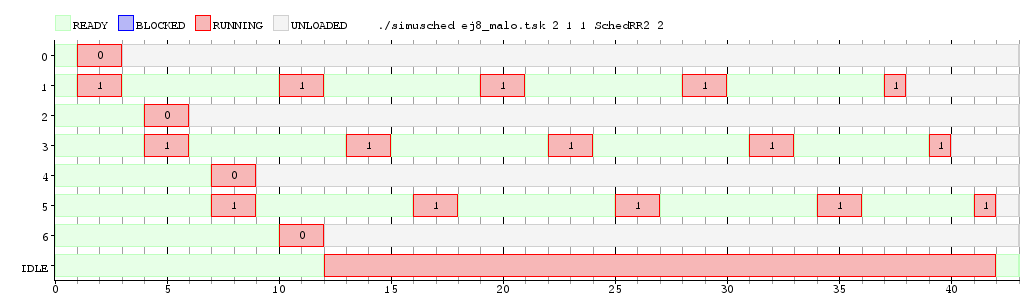
\includegraphics[width=1\textwidth]{ej8MaloRR2}
    \caption{Ejecución en Round-Robin 2}
    \label{RR2Malo}
\end{figure}

Como se muestra en la figura \ref{RR2Malo}, podemos notar lo antes mencionado. Con este nuevo scheduler, a partir del instante 16, el CPU 0, ya no posee ninguna tarea a ejecutar, siendo que terminaron todas las que fueron asignadas al mismo al momento de carga. Por lo tanto, queda en IDLE, mientras que el CPU 1 ejecuta alternadamente los 3 procesos restantes.

% Tabla RR2
\begin{table}[h]
  \begin{center}
    \begin{tabular}{c c c c c}
    \hline
          & Latencia & Espera & Compleción & Ratio (E/C) \\
    \hline
        0 &     1    &    1   &      3     &     0.333   \\
        1 &     1    &   29   &     38     &     0,763   \\
        2 &     4    &    4   &      6     &     0.666   \\
        3 &     4    &   31   &     40     &     0.775   \\
        4 &     7    &    7   &      9     &     0.777   \\
        5 &     7    &   33   &     42     &     0,785   \\
        6 &     10   &   10   &     12     &     0.833   \\
        AVG & 4,857  & 16,428 &   21,428   &     0,705   \\
    \end{tabular}
  \end{center}
\end{table}

\begin{figure}[h]
    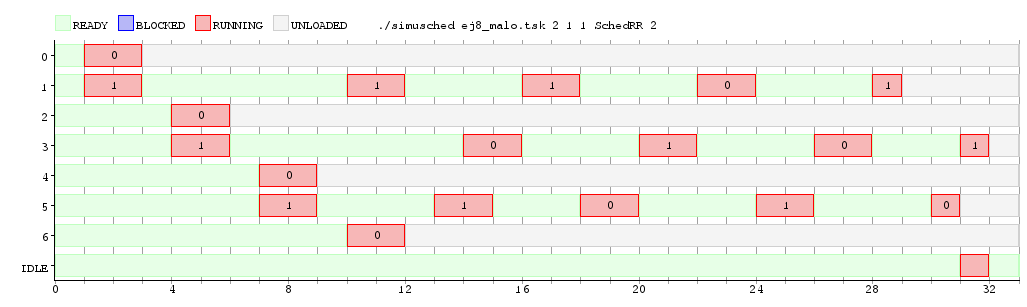
\includegraphics[width=1\textwidth]{ej8MaloRR}
    \caption{Ejecución en Round-Robin Tradicional}
    \label{RRMalo}
\end{figure}

En cambio, en la figura \ref{RRMalo}, podemos observar, como con el Round-Robin tradicional, cuando terminan de ejecutarse las tareas cortas (0, 2, 4 y 6), el CPU 1 sigue siendo utilizado por las restantes. Notar que aunque perdemos 1 ciclo extra por cambio de CPU, los procesos siguen terminando antes que con el nuevo scheduler implementado.

% Tabla RR1
\begin{table}[h]
  \begin{center}
    \begin{tabular}{c c c c c}
    \hline
          & Latencia & Espera & Compleción & Ratio (E/C) \\
    \hline
        0 &     1    &    1   &      3     &    0.333    \\
        1 &     1    &   20   &     29     &    0,690    \\
        2 &     4    &    4   &      6     &    0.666    \\
        3 &     4    &   23   &     32     &    0,719    \\
        4 &     7    &    7   &      9     &    0.777    \\
        5 &     7    &   22   &     31     &    0,710    \\
        6 &     10   &   10   &     12     &    0.833    \\
        AVG & 4,857  & 12,429 &   17,428   &    0,675    \\
    \end{tabular}
  \end{center}
\end{table}


Sin embargo, este nuevo tipo de scheduler resulta útil en algunas situaciones. Tal es el caso cuando se desea (...)

Por ejemplo, en arquitecturas SMP, es importante mantener cierta afinidad al procesador asignado al proceso, para aprovechar la caché. Si hubiera cambio de procesador, el proceso llegaría con la caché vacía, produciéndose un miss y teniendo que ir a buscar los datos a memoria principal. A esto se le suma el tiempo de los cambios de procesador y de contexto.



%Una forma de mitigar el problema antes mencionado sería intentar "balancear" la cantidad de procesos para cada CPU, moviendo procesos cuando haya lugar en otros núcleos, pero manteniendo cierta afinidad

% Latencia
% Espera
% Compleción
% Ratio (E/C)

% Cualquier esquema de prioridades fijas corre riesgo de inanicion.
% Si el quantum es muy corto, el tiempo de scheduling+context switch se vuelve una proporción importante del quantum. Por ende, el sistema pasa un porcentaje alto de su tiempo haciendo “mantenimiento” en lugar de trabajo de verdad.
% La idea general es minimizar el tiempo de respuesta para los procesos interactivos, suponiendo que los cómputos largos son menos sensibles a demoras.
